\documentclass[tikz,border=6pt]{standalone}
\usepackage[T1]{fontenc}
\usepackage{helvet}
\renewcommand{\familydefault}{\sfdefault}
\usetikzlibrary{arrows.meta}
\tikzset{
  box/.style={draw,thick,minimum width=3.6cm,minimum height=1.4cm,align=center,font=\small},
  arr/.style={-{Stealth[length=2.5mm]},thick},
  lab/.style={font=\scriptsize}
}
\begin{document}
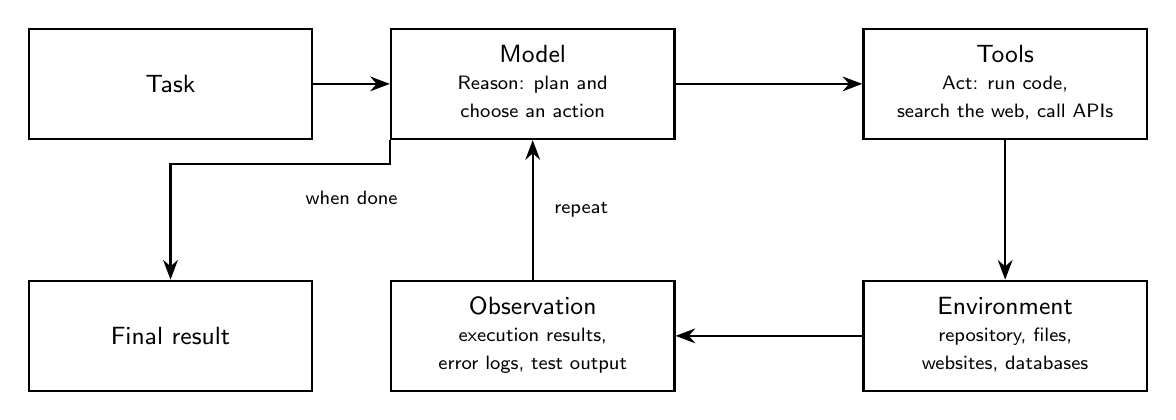
\begin{tikzpicture}
  \node[box] (task) at (-4.6,1.6) {Task};
  \node[box] (model) at (0,1.6) {\begin{tabular}{c}
      Model\\[-1pt]
      {\scriptsize Reason: plan and}\\[-1pt]
      {\scriptsize choose an action}
    \end{tabular}};
  \node[box] (tool) at (6,1.6) {\begin{tabular}{c}
      Tools\\[-1pt]
      {\scriptsize Act: run code,}\\[-1pt]
      {\scriptsize search the web, call APIs}
    \end{tabular}};
  \node[box] (env) at (6,-1.6) {\begin{tabular}{c}
      Environment\\[-1pt]
      {\scriptsize repository, files,}\\[-1pt]
      {\scriptsize websites, databases}
    \end{tabular}};
  \node[box] (obs) at (0,-1.6) {\begin{tabular}{c}
      Observation\\[-1pt]
      {\scriptsize execution results,}\\[-1pt]
      {\scriptsize error logs, test output}
    \end{tabular}};
  \node[box] (out) at (-4.6,-1.6) {Final result};

  \draw[arr] (task) -- (model);
  \draw[arr] (model) -- (tool);
  \draw[arr] (tool) -- (env);
  \draw[arr] (env) -- (obs);
  \draw[arr] (obs) -- (model);
  \draw[arr] (model.south west) -- ++(0,-0.3) -| (out.north);
  \node[lab,anchor=west] at (0.15,0) {repeat};
  \node[lab] at (-2.3,0.15) {when done};
\end{tikzpicture}
\end{document}
